\documentclass[11pt,a4paper]{article}

% PACKAGES
% ============================================================
\usepackage[utf8]{inputenc}
\usepackage{placeins}
\usepackage{hyperref}
\usepackage[T1]{fontenc}
\usepackage[english]{babel}
\usepackage{amsmath,amssymb,amsfonts}
\usepackage{graphicx}
\usepackage{float}
\usepackage{booktabs}
\usepackage{array}
\usepackage{fancyhdr}
\usepackage{hyperref}
\usepackage{tikz}
\usepackage[all]{hypcap}
\usepackage{times}       % Times New Roman-style font, matching the original docx
\usepackage{cancel}      % for striking out terms (as used in the original report)
\usepackage{caption}
\usepackage{subcaption}
\usepackage{xcolor}
\usepackage{listings}
\usepackage{needspace}
\usepackage{amsmath}

\lstset{
    language=Matlab,
    basicstyle=\ttfamily\small,
    numbers=left,
    numberstyle=\tiny,
    frame=single,
    breaklines=true,
    showstringspaces=false
}
\usetikzlibrary{arrows.meta, positioning, calc}

% ============================================================
% MARGINS
% Values measured directly from the reference PDF (real position
% of the text boxes relative to the page edges, across several
% content pages):
%   left / right         ~ 1.02 cm
%   top (down to header) ~ 0.68 cm
%   header -> body text  ~ 0.62 cm
%   body text -> footer  ~ 0.8-1.1 cm
%   footer -> page bottom~ 0.82 cm
% ============================================================
\usepackage[
    a4paper,
    left=1cm,
    right=1cm,
    top=0.5cm,
    bottom=0.45cm,
    headheight=14pt,
    headsep=0.3cm,
    footskip=0.85cm,
    includeheadfoot
]{geometry}

\graphicspath{{figs/}}

% Compact spacing
\captionsetup{font=small,skip=2pt}
\setlength{\abovedisplayskip}{2pt}
\setlength{\belowdisplayskip}{2pt}
\setlength{\abovedisplayshortskip}{0pt}
\setlength{\belowdisplayshortskip}{0pt}
\setlength{\textfloatsep}{4pt}

% Notation
\newcommand{\vect}[1]{\boldsymbol{#1}}
\newcommand{\Sk}[1]{S(#1)}            % skew-symmetric matrix
\newcommand{\hatx}{\hat{\vect{x}}}

\begin{document}

\section{Model and filter}
\label{sec:model}

In the paper~\cite{batista2011} the measurement $\vect{y}(t)=\mathcal{R}^{\mathsf T}(t)\,{}^{I}\vect{y}$ is the observation of a constant vector ${}^{I}\vect{y}$ in the inertial frame, with $\mathcal{R}$ the rotation from the body to the inertial frame.
Here that vector is gravity, ${}^{I}\vect{y}=[0\;0\;{-g}]^{\mathsf T}$ (this accelerometer reads $a_z=-g$ at rest), so $\vect{y}$ is the accelerometer reading.
The input is the gyro measurement $\vect{\omega}_m=\vect{\omega}+\vect{b}$, and the state is $\vect{x}=[\vect{x}_1^{\mathsf T}\;\vect{x}_2^{\mathsf T}]^{\mathsf T}=[\vect{y}^{\mathsf T}\;\vect{b}^{\mathsf T}]^{\mathsf T}\in\mathbb{R}^6$: the gravity vector in body axes and the gyro bias.

The system (2) of the paper is $\dot{\vect{x}}=A(t)\vect{x}$, $\vect{y}=C\vect{x}$, with $C=[I\;0]$.
Unlike a steady-state filter, $A(t)$ depends on the measured $\vect{y}$ and $\vect{\omega}_m$ and must be recomputed at every iteration, so the Kalman gain is no longer stationary and the Riccati equation has to be solved online,
\begin{equation}
\dot P = A(t)P + PA(t)^{\mathsf T} + Q - PC^{\mathsf T}R^{-1}CP, \qquad K(t) = P(t)C^{\mathsf T}R^{-1},
\label{eq:riccati}
\end{equation}
where $Q$ and $R$ are the process and measurement noise intensities.
The system is observable if $\vect{y}(t)$ changes direction (Theorems 3.3 and 3.4 of the paper), so with the drone at rest the bias along gravity is not observable, and a single vector observation only gives roll and pitch:
\begin{equation}
\hat\phi = \operatorname{atan2}(-\hat x_2,\,-\hat x_3), \qquad
\hat\theta = \arcsin\!\big(\hat x_1 / \|\hat{\vect{x}}_1\|\big).
\label{eq:angles}
\end{equation}

\section{Implementation and tuning}
\label{sec:impl}

The filter \eqref{eq:riccati} runs in continuous time in Simulink, with a fixed-step solver at the sample time of the data.
The Simulink model is shown in Fig.~\ref{fig:sim_model} (Appendix~\ref{app:simulink}), and the same model is used in simulation and in replay.

The noise intensities are built from the sensor statistics of Section~3 of the guide~\cite{guia} in hover, with $\sigma_g$ and $\sigma_a$ the standard deviations of the gyros and of the accelerometer,
\begin{equation}
Q = \begin{bmatrix} (g\sigma_g)^2 T_s\, I_3 & 0 \\ 0 & q_b\, I_3 \end{bmatrix}, \qquad
R = \alpha\,\sigma_a^2\, T_s\, I_3.
\label{eq:tuning}
\end{equation}
The gyro noise enters multiplied by $\vect{y}$, which explains the factor $g$ in $Q$, and $q_b$ is the random walk of the bias.
The factor $\alpha>1$ lowers the trust in the accelerometer, because in flight its error is vibration and linear acceleration and not white noise.
The filter starts level with zero bias and a large uncertainty on the accelerometer states.
The parameters $\alpha$ and $q_b$ were chosen by a sweep that minimises the error against the onboard estimator in D and E (Table~\ref{tab:sens}).

\section{Results}
\label{sec:results}

\subsection{Simulation with known truth}

The simulation uses sinusoidal roll and pitch at different frequencies, so that $\vect{y}$ keeps changing direction, with Gaussian sensor noise and a constant gyro bias.
The errors are computed after the initial transient.

\begin{figure}[htbp]
\centering
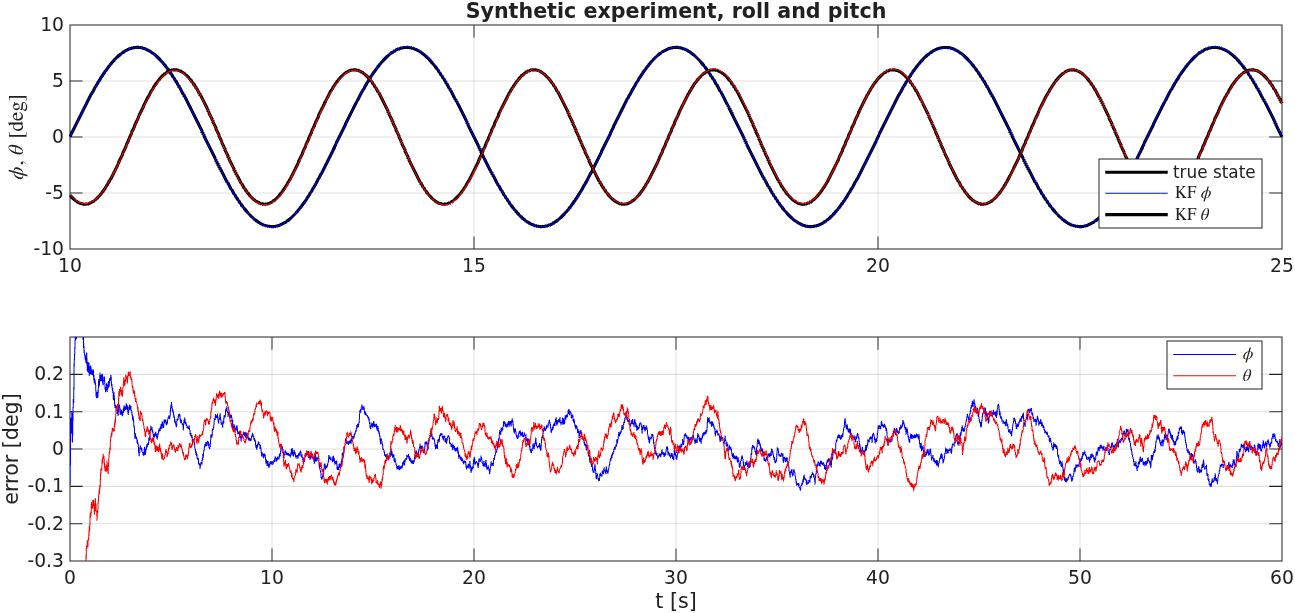
\includegraphics[width=0.58\linewidth]{fig_sim}
\caption{Synthetic experiment (ideal case). Top: true roll and pitch (black) and estimated roll and pitch (blue and red), from 10 to 25~s. Bottom: attitude error (the first 3~s fall outside the axes).}
\label{fig:sim_att}
\end{figure}

\begin{table}[htbp]
\caption{Synthetic experiment: error after 10 s and estimated bias}
\label{tab:sim}
\centering
\begin{tabular}{lccc}
\hline
Case & RMS $\phi/\theta$ (deg) & $\bar e$ $\phi/\theta$ (deg) & $\hat{\vect{b}}$ (deg/s) \\
\hline
Default & 0.05 / 0.05 & +0.01 / 0.00 & [2.01, $-$3.01, 0.96] \\
Accelerometer bias & 0.98 / 0.20 & +0.98 / $-$0.19 & [2.01, $-$3.01, 0.89] \\
Noise $\times 0.01$ & 0.03 / 0.03 & 0.00 / 0.00 & [2.00, $-$3.00, 0.93] \\
\hline
\end{tabular}
\end{table}

In Fig.~\ref{fig:sim_att} the estimate overlaps the truth on both axes, and the error is a few hundredths of a degree after a transient of about 3~s (Table~\ref{tab:sim}).
The gyro bias is recovered on all three axes (Fig.~\ref{fig:bias}, top).
A constant accelerometer bias produces a constant offset in $\phi$ and $\theta$ that the filter does not correct (Table~\ref{tab:sim}, row 2: 0.98\textdegree{} in $\phi$ for a bias of $[-0.033,-0.166,0]$~m/s$^2$), because with a single vector measurement it is indistinguishable from a tilt.

\begin{figure}[htbp]
\centering
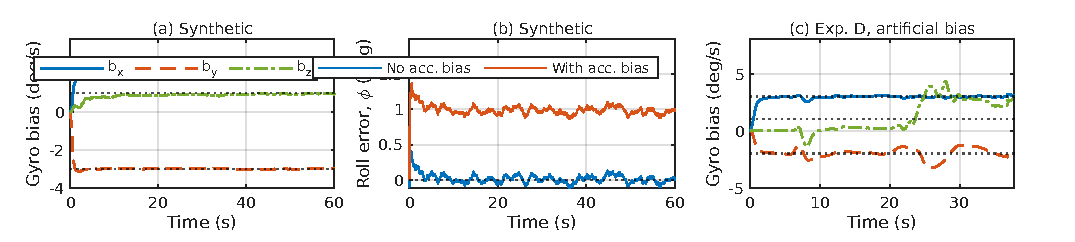
\includegraphics[width=0.58\linewidth]{fig_bias}
\caption{Gyro bias estimate (colour) and true bias (black). Top: synthetic experiment. Bottom: experiment D with an artificial bias of $[3,\,-2,\,1]$~deg/s added to the gyros.}
\label{fig:bias}
\end{figure}

\subsection{Real data}

There is no ground truth in experiments C (hover), D (pitch steps) and E ($y$ mission), so the filter is compared with the attitude estimated onboard by the drone, for $t>10$~s and $t<t_f-3$~s.

\begin{figure}[htbp]
\centering
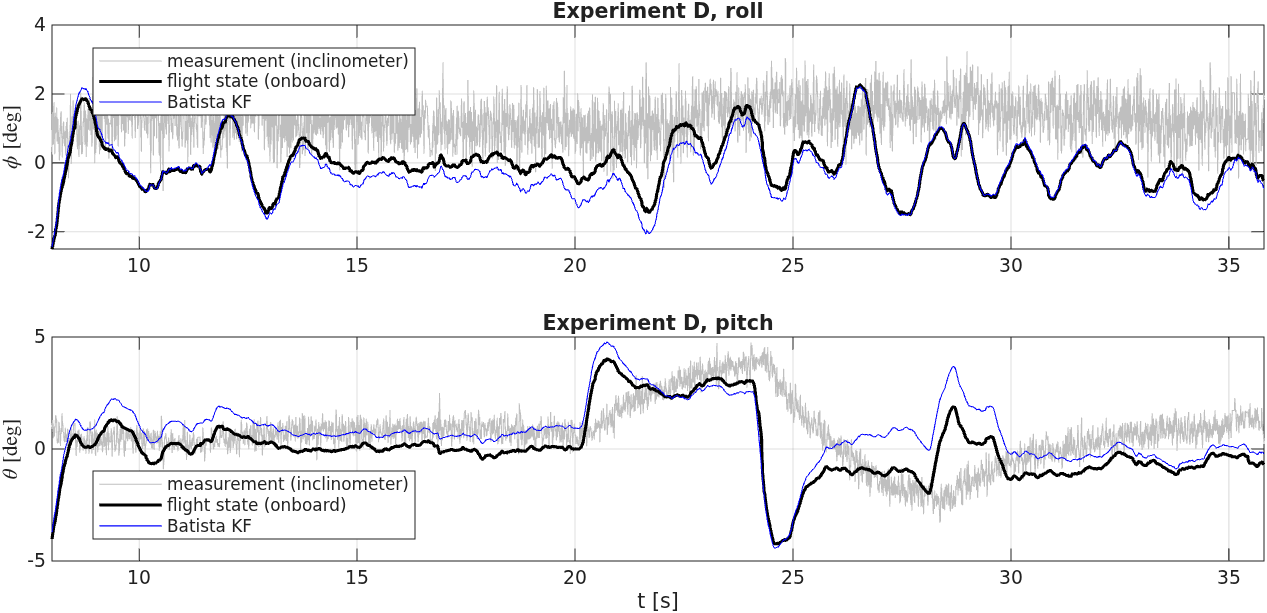
\includegraphics[width=0.58\linewidth]{fig_real_D}
\caption{Experiment D (pitch steps). Roll and pitch: inclinometer (grey), onboard estimator (black) and Batista filter (blue).}
\label{fig:real_D}
\end{figure}
\begin{figure}[htbp]
\centering
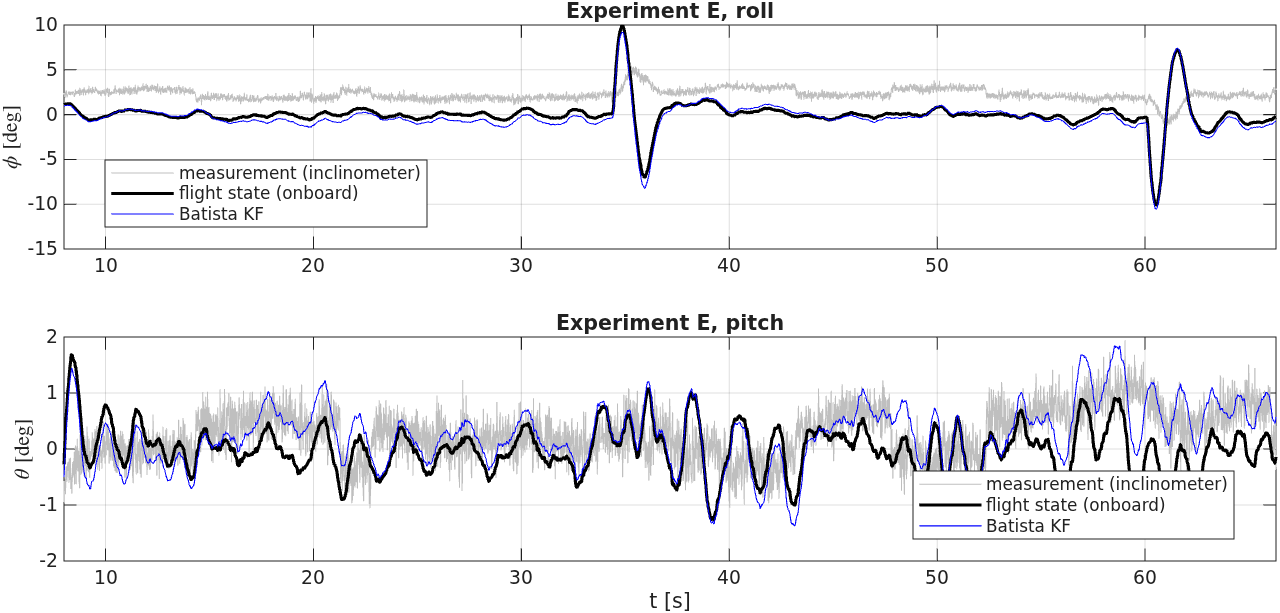
\includegraphics[width=0.58\linewidth]{fig_real_E}
\caption{Experiment E ($y$ mission). Roll and pitch: inclinometer (grey), onboard estimator (black) and Batista filter (blue).}
\label{fig:real_E}
\end{figure}

\begin{table}[htbp]
\caption{Real data against the onboard estimator (standard deviation / mean of the error, in deg; $\phi/\theta$)}
\label{tab:real}
\centering
\begin{tabular}{lcccc}
\hline
Exp. & Std incl. & Std filter & Mean incl. & Mean filter \\
\hline
C & 0.55 / 0.45 & 0.11 / 0.11 & +2.14 / +0.95 & +0.40 / +0.57 \\
D & 0.89 / 1.59 & 0.24 / 0.55 & +1.30 / +0.62 & $-$0.24 / +0.71 \\
E & 1.83 / 0.57 & 0.41 / 0.37 & +2.25 / +0.31 & $-$0.31 / +0.28 \\
\hline
\end{tabular}
\end{table}

Figs.~\ref{fig:real_D} and~\ref{fig:real_E} and Table~\ref{tab:real} lead to three conclusions.
First, the filter removes most of the inclinometer noise: the grey measurement is very noisy even in hover, and the standard deviation of the error against the onboard estimator drops by a factor of 1.5 to 5 (for example, pitch in D goes from 1.59\textdegree{} to 0.55\textdegree).
Second, the filter follows the manoeuvres with the right amplitude and without visible delay, in the pitch steps of D and in the roll of E, because the fast part comes from the gyros and the inclinometer only corrects the slow drift.
Third, the remaining error is concentrated in the manoeuvres, where it reaches about 2\textdegree, and is flat in hover (standard deviation of 0.11\textdegree), because the accelerometer reads linear acceleration as tilt and the model ignores it.
There is also a constant offset of a few tenths of a degree in the filter, against about 2\textdegree{} in the roll inclinometer, which comes from the accelerometer bias and varies between experiments, and part of it may come from the onboard estimator, which is not the truth either.

\subsection{Gyro bias}

The real gyro bias is close to zero (mean at rest of $[-0.03,\,-0.02,\,0.01]$~deg/s), so, as the guide suggests~\cite{guia}, $[3,-2,1]$~deg/s was added to the gyros of experiment D (Fig.~\ref{fig:bias}, bottom).
Within a few seconds the $x$ and $y$ components converge to $3.11$ and $-2.06$~deg/s.
The $z$ component stays at $2.74$~deg/s, far from $1$~deg/s, because it is only observable when the drone rotates, which hardly happens in D.

\subsection{Sensitivity to the tuning}
\label{sec:sens}

\begin{table}[htbp]
\caption{Error (deg) for different values of $\alpha$ and $q_b$ (RMS in the synthetic case, standard deviation against the onboard estimator in D and E, $\phi$ and $\theta$ combined). Adopted values in bold; ``div.'' means that the simulation diverges.}
\label{tab:sens}
\centering
\setlength{\tabcolsep}{6pt}
\begin{tabular}{l cccccc}
\toprule
 & \multicolumn{6}{c}{Measurement noise factor $\alpha$} \\
\cmidrule(lr){2-7}
 & $1$ & $10$ & $10^{2}$ & $\mathbf{10^{3}}$ & $10^{4}$ & $10^{5}$ \\
\midrule
Synthetic & div. & div. & div. & \textbf{0.05} & 0.06 & 0.30 \\
Exp.\ D   & div. & div. & div. & \textbf{0.42} & 0.64 & 0.85 \\
Exp.\ E   & div. & div. & div. & \textbf{0.39} & 0.44 & 0.48 \\
\midrule
 & \multicolumn{6}{c}{Bias random walk $q_b$} \\
\cmidrule(lr){2-7}
 & $10^{-8}$ & $10^{-7}$ & $10^{-6}$ & $\mathbf{10^{-5}}$ & $10^{-4}$ & \\
\midrule
Synthetic & 0.07 & 0.06 & 0.05 & \textbf{0.05} & 0.05 & \\
Exp.\ D   & 0.81 & 0.76 & 0.60 & \textbf{0.42} & 0.76 & \\
Exp.\ E   & 0.45 & 0.46 & 0.43 & \textbf{0.39} & 0.51 & \\
\bottomrule
\end{tabular}
\end{table}

The adopted $q_b$ is the minimum in D and E (Table~\ref{tab:sens}).
For $\alpha\le100$ the simulation diverges: a small $R$ makes the gain $K=PR^{-1}$ too large for the fixed-step Euler solver, which becomes numerically unstable.

\section{Limitations and conclusion}
\label{sec:limits}

The real reference is the drone's onboard estimator, not the truth, so only the simulation measures absolute error.
The parameters $\alpha$ and $q_b$ were chosen on D and E, which are also evaluated, while C did not take part in the choice.
The gyro bias in $z$ is only reliable if the drone rotates: in D and E it is estimated at $1.74$ and $-1.97$~deg/s, when the real value is close to zero.

The Batista et al.\ filter estimates roll and pitch with an error of 0.05\textdegree{} RMS in simulation and a standard deviation of 0.11\textdegree{} to 0.55\textdegree{} against the onboard estimator on real data, 1.5 to 5 times less than the inclinometer, and it recovers the gyro bias when the drone excites the system.
The remaining error comes from the accelerometer bias and from the linear acceleration during manoeuvres, which the model does not handle.

\begin{thebibliography}{1}
\bibitem{batista2011}
P.~Batista, C.~Silvestre, and P.~Oliveira, ``Partial attitude and rate gyro bias estimation: observability analysis, filter design, and performance evaluation,'' \emph{Int.\ J.\ Control}, vol.~84, no.~5, pp.~895--903, May 2011.

\bibitem{guia}
Instituto Superior T\'ecnico, ``Laboratory 2 guide: Estimation,'' Aeronaves Robotizadas, MEAer, 2026/27.
\end{thebibliography}

\appendix
\section{Simulink diagram}
\label{app:simulink}

\begin{figure}[htbp]
\centering
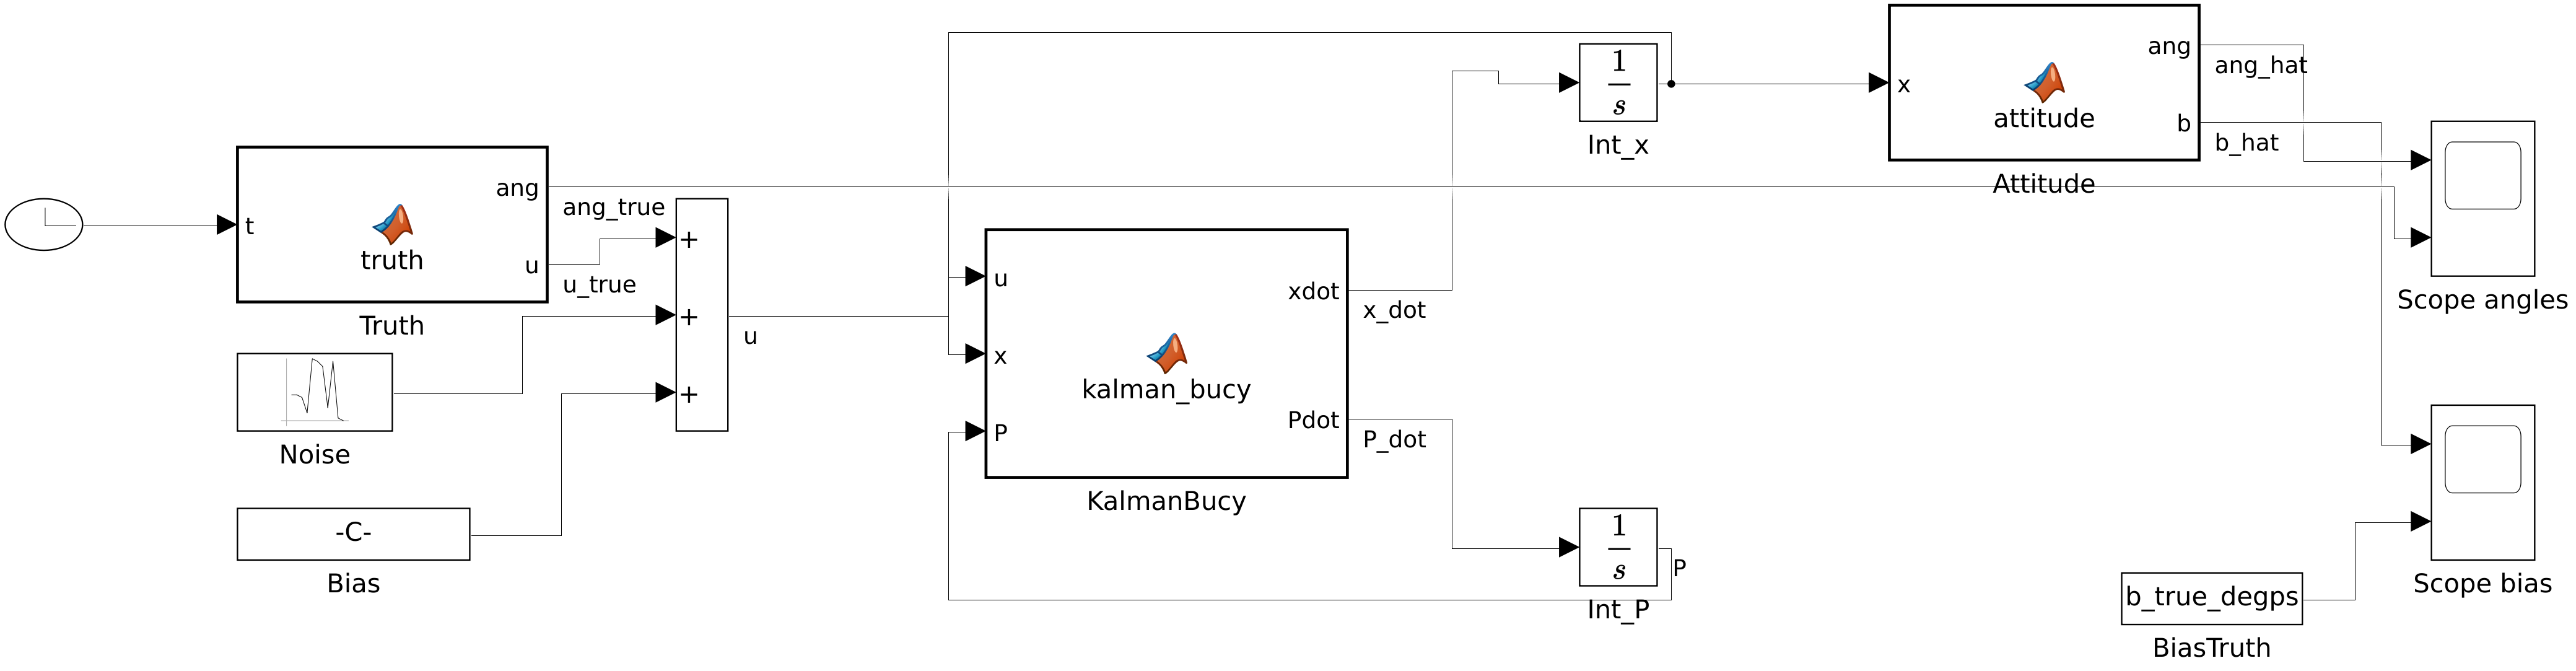
\includegraphics[width=\linewidth]{simulink_sim}
\caption{Simulink model of the filter (simulation version). The model has four blocks: \texttt{KalmanBucy} computes $\dot{\hatx}$ and $\dot P$ from \eqref{eq:riccati}, the integrators \texttt{Int\_x} and \texttt{Int\_P} close the loop, and \texttt{Attitude} applies \eqref{eq:angles}. In simulation, \texttt{Truth} generates the exact roll, pitch and sensor readings, and \texttt{Noise} and \texttt{Bias} corrupt them. In replay, \texttt{Truth}, \texttt{Noise} and \texttt{Bias} are replaced by the recorded data, and the onboard estimator of the drone is used as reference.}
\label{fig:sim_model}
\end{figure}

\end{document}
